\documentclass{../cssheet}
%--------------------------------------------------------------------------------------------------------------
% Basic meta data
%--------------------------------------------------------------------------------------------------------------

\title{Mengen in Präsenz}
\author{Prof. Dr. Christian Spannagel}
\date{\today}
\hypersetup{%
    pdfauthor={\theauthor},%
    pdftitle={\thetitle},%
    pdfsubject={Aufgabenblatt Inside Math!},%
    pdfkeywords={insidemath}
}

%--------------------------------------------------------------------------------------------------------------
% document
%--------------------------------------------------------------------------------------------------------------

\begin{document}
\printtitle

\vspace*{10mm}


\textbf{Aufgabe 1 (Lieber direkt als um die Ecke):}  Findet Mengen $A$, $B$, $C$ und $D$ so, dass das folgende Venn-Diagramm stimmt.

\begin{center}
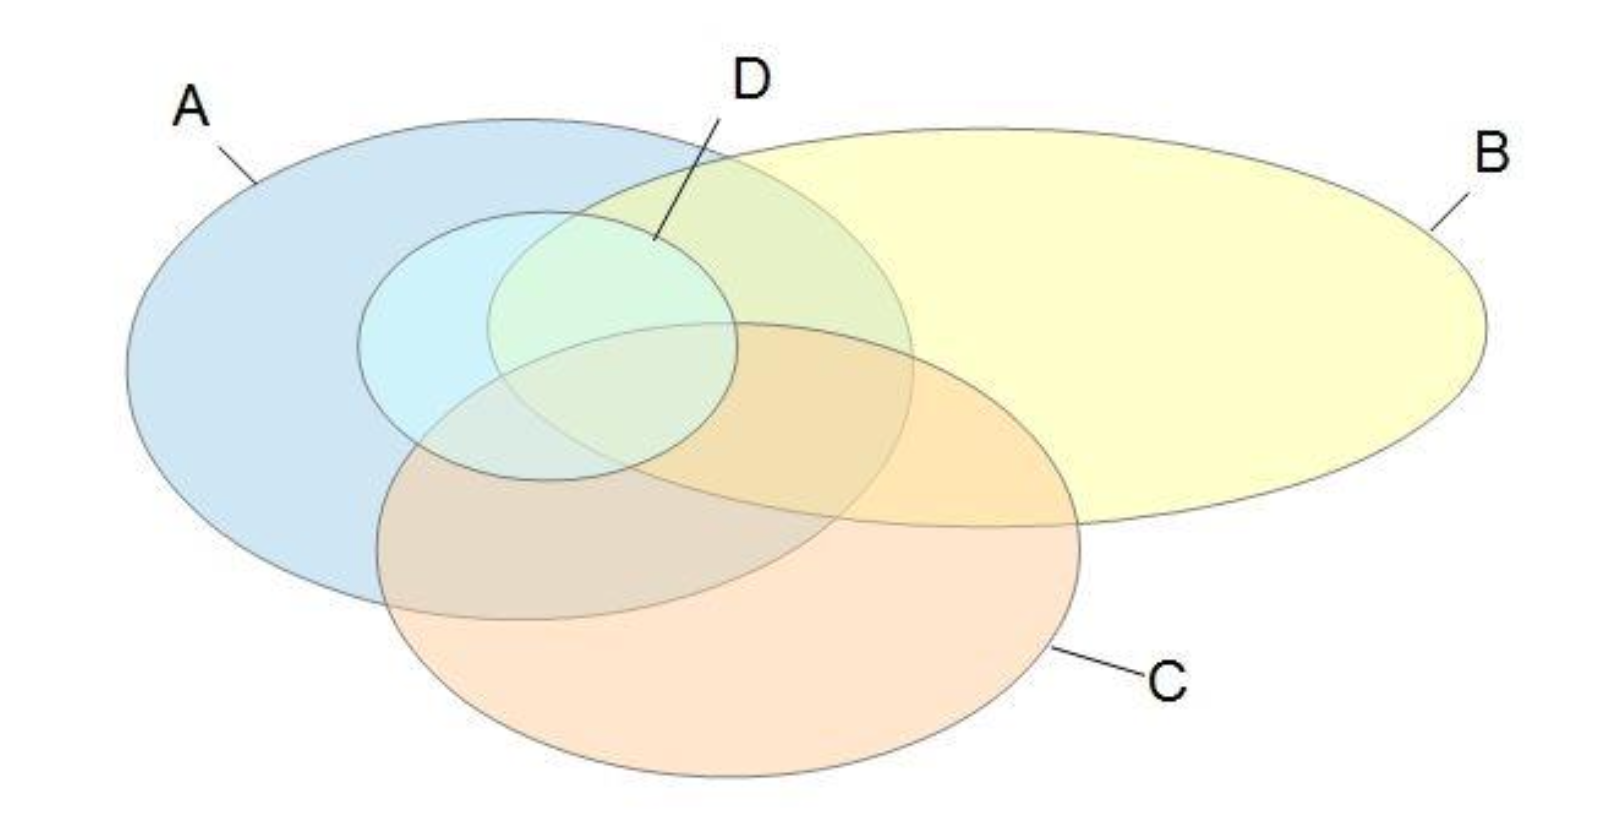
\includegraphics[width=10cm]{venn.png}
\end{center}


\textbf{Aufgabe 2 (Ich spring im Dreieck):} Wie hängen die folgenden Mengen zusammen?
Stellt eure Überlegungen jeweils graphisch mit Hilfe von Venn-Diagrammen dar!

\begin{itemize}
\item die Menge aller gleichschenkligen Dreiecke
\item die Menge aller Dreiecke
\item die Menge aller gleichseitigen Dreiecke
\item die Menge aller rechtwinkligen Dreiecke
\item die Menge aller gleichwinklingen Dreiecke
\end{itemize}

\vspace*{10mm}
%\newpage
\printlicense

\printsocials

\end{document}
